\chapter{Vision and goals}
\section{Hj{\o}rring Library: a place for experiences}\label{hjoerring}
In this chapter we will investigate the target group for the project. A preliminary assessment will be made to gather information that will help towards making the program suit the target group best.

Hj{\o}rring Library aims to distinguish itself from most other Danish libraries. The first distinguishing factor is the location of the library: a big shopping mall. Inside, visitors find themselves in a big open hall with modern architecture. The different sections are divided by bookshelves and a red stripe that runs throughout the library (called "den r{\o}de tr{\aa}d"). While the library first and foremost is a library as any other, one of the prevalent feelings that visitors get is that Hj{\o}rring Library is a place to "hang out" and relax (see figure \ref{fig:p1}), but also a place to have fun or do some work. There are many unique pieces of furniture, creating a great environment for all purposes. Especially kids can have a fun time playing games (physical or digital) and recording videos in the children zone (see figures \ref{fig:p2} and \ref{fig:p3}).

At Hj{\o}rring Library the staff has made a big effort to create an environment as interactive as possible, with many places for people to entertain themselves with other things than just traditional books. Even the cafeteria appears to be part of the library's ordinary environment where people can show up, eat their lunch, drink coffee or just have a beer after work.

\begin{figure}[htbp]\centering
	\begin{minipage}[b]{0.3\textwidth}\centering
		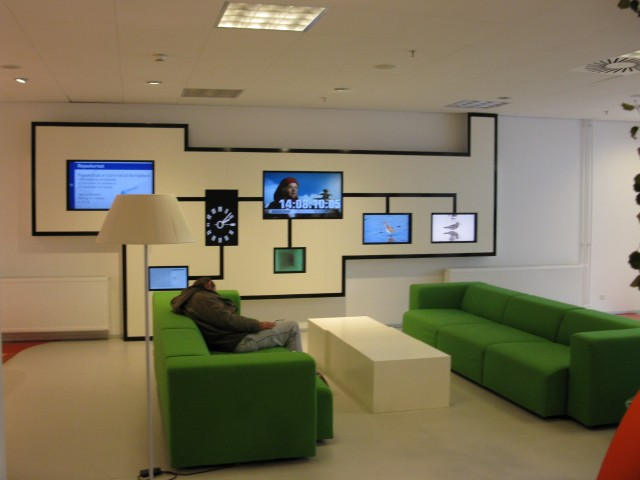
\includegraphics[width=1.00\textwidth]{Pictures/HjoerringLibrary/p1.jpg} %Venstre billede
	\end{minipage}\hfill
	\begin{minipage}[b]{0.3\textwidth}\centering
		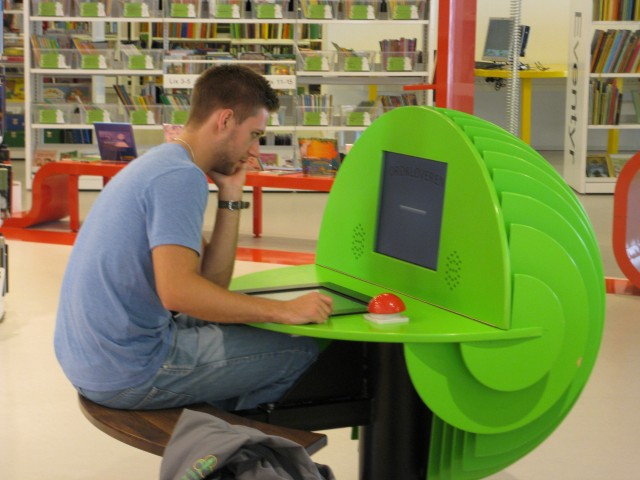
\includegraphics[width=1.00\textwidth]{Pictures/HjoerringLibrary/p2.jpg} %Venstre billede
	\end{minipage}\hfill	
	\begin{minipage}[b]{0.3\textwidth}\centering
		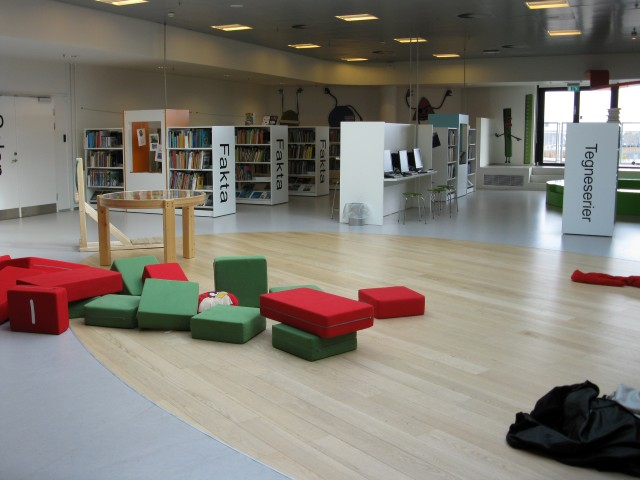
\includegraphics[width=1.00\textwidth]{Pictures/HjoerringLibrary/p3.jpg} %Højre billede
	\end{minipage}\\ %Captions and labels
	\begin{minipage}[t]{0.3\textwidth}
		\caption{Lounge.} %Venstre caption og label
		\label{fig:p1}
	\end{minipage}\hfill
	\begin{minipage}[t]{0.3\textwidth}
		\caption{Playing games.} %Venstre caption og label
		\label{fig:p2}
	\end{minipage}\hfill	
	\begin{minipage}[t]{0.3\textwidth}
		\caption{Physical Angry Birds game} %Højre caption og label
		\label{fig:p3}
	\end{minipage}
\end{figure}

Hj{\o}rring Library is popular for giving new and exiting experiences to its visitors. One way to achieve this is by having various themes that run throughout the whole library. These includes topics such as: Arabia, birds, fairy tales or simply the color brown. In the period of this project, Hj{\o}rring library has chosen the topic of Christmas, and it will run from the second week of November until the last week of December, 2012. At the time of the first visit to the library, a bird-theme was running. All kinds of birds were exhibited around the library (see figures \ref{fig:b1} and \ref{fig:b2}), and bird songs were played on several hidden speakers.

\begin{figure}[htbp]\centering
	\begin{minipage}[b]{0.48\textwidth}\centering
		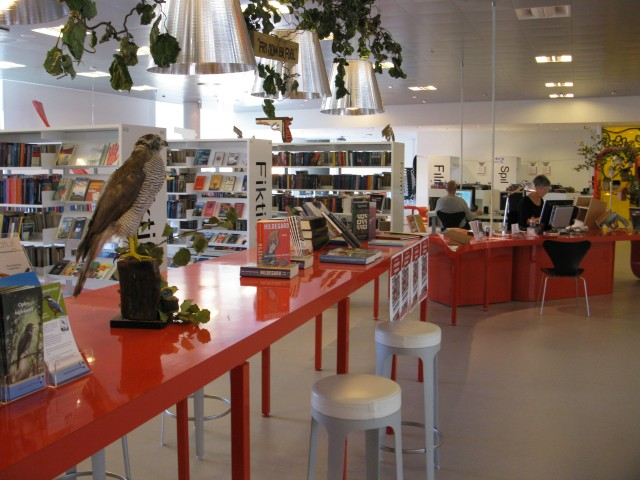
\includegraphics[width=1.00\textwidth]{Pictures/HjoerringLibrary/b1.jpg} %Venstre billede
	\end{minipage}\hfill
	\begin{minipage}[b]{0.48\textwidth}\centering
		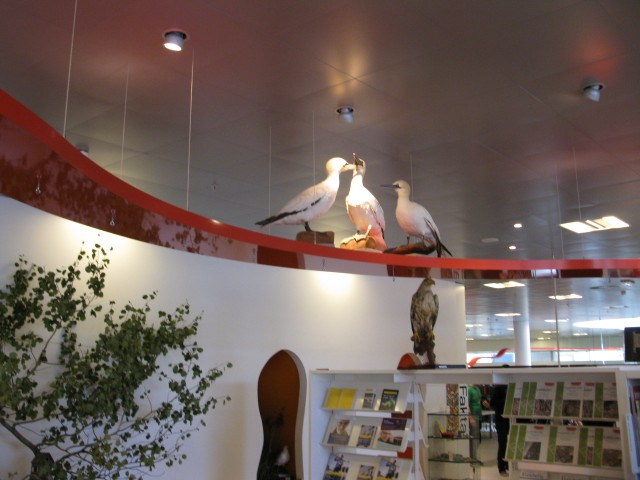
\includegraphics[width=1.00\textwidth]{Pictures/HjoerringLibrary/b2.jpg} %Højre billede
	\end{minipage}\\ %Captions and labels
	\begin{minipage}[t]{0.48\textwidth}
		\caption{Birds.} %Venstre caption og label
		\label{fig:b1}
	\end{minipage}\hfill
	\begin{minipage}[t]{0.48\textwidth}
		\caption{More birds.} %Højre caption og label
		\label{fig:b2}
	\end{minipage}
\end{figure}

These themes are an example of how Hj{\o}rring Library tries to work with the concept of \textit{serendipity}, which basically describes a happy accident; something you did not expect but turned out to be a pleasant surprise. Even though you go to the library to find a book, you might also experience and learn something that you originally did not expect.

Hj{\o}rring Library is always looking for new projects to involve its visitors in new and engaging ways. Since some Medialogy students previously came to the library to do projects and they turned out to be successful, the staff is eager to try it out again. This is where our group comes into the picture. To us, this is a great opportunity to collaborate with an institution on a project in a real-life setting. Instead of only testing under artificial circumstances, the library will allow us to test on visitors at the library throughout December.

Generally the atmosphere at the library is the same as that of any other library, as such the visitors (mainly students and adult visitors) naturally expect a quiet and calm working area.

\subsection{Considerations}
The goal for the program is to fit into the library without disturbing visitors, who do not wish to interact with the installation. This means that the program should not emit loud sounds that disturb visitors.

In order for the installation to be a fun experience for both a passive and an active user, the program will function on more than one level. An active user is a user that actively interacts with the canvas, and a passive is a someone who just walks by. This means that you should be able to pass by and admire the installation and also be able to spend more time in front of it.

\subsection{Visitor data and placement of the canvas}
The library is divided into several parts, each aiming to give a different experience. It is important for the group to get a central location for the placement of the canvas. This ensures that people will have the chance to interact with the program. In fact, the bookshelves chosen are just in the middle of the library, so it is hard not to walk past it at some point (see figure \ref{fig:library_floorplans}).

\begin{figure}[htbp]
\centering
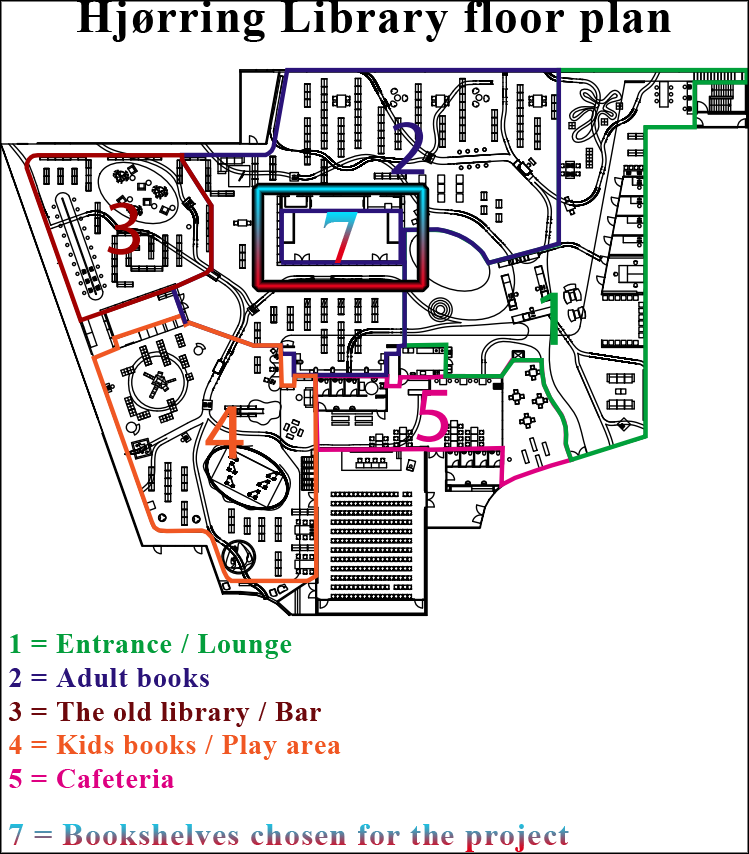
\includegraphics[width=0.80\textwidth]{Pictures/HjoerringLibrary/hjoerring_library_floorplans.png}
\caption{Hj{\o}rring Library is divided into multiple sections. We chose to use a big four-sided bookshelf in the core of the library. Image inspired by \citep{hjoerring_study}.}
\label{fig:library_floorplans}
\end{figure}

%%%%%%%%%%%%%%%%%%%%%%% \citep{hjoerring_study} is shown as [hjo]!!!!!!!!!!!!!!!! %%%%%%%%%%%%%%%%%%%%%%%%

In 2010 \citep{hjoerring_study} did a survey to investigate people's habits and movement patterns at Hj{\o}rring Library. They found that an average visitor spends about half an hour at the library. Those in the age group between 0-10 years and 21-30 years spent the most time at the library, 34 and 44 minutes, while those between 41-50 and 61-70 years spent 19 and 26 minutes during an average visit.

Several cylinder and flow maps were made to visualize the gathered data. Two are shown in figures \ref{fig:library_cylindermap} and \ref{fig:library_flowmap}.

\begin{figure}[htbp] \centering
\begin{minipage}[b]{0.45\textwidth} \centering
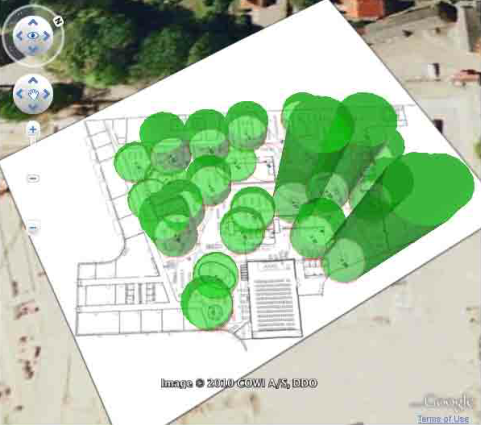
\includegraphics[width=1.00\textwidth]{Pictures/HjoerringLibrary/library_cylinder_diagram_24Nov.png} % Venstre billede
\end{minipage} \hfill
\begin{minipage}[b]{0.45\textwidth} \centering
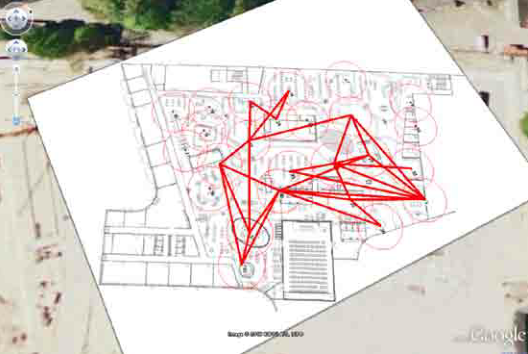
\includegraphics[width=1.00\textwidth]{Pictures/HjoerringLibrary/library_flow_Nov21.png} % Højre billede
\end{minipage} \\ % Captions og labels
\begin{minipage}[t]{0.45\textwidth}
\caption{Cylinder map showing multiple visitor's accumulated visiting time at Hj{\o}rring Library Tuesday November 24, 2010. Image created by \citep{hjoerring_study}.} % Venstre caption og label
\label{fig:library_cylindermap}
\end{minipage} \hfill
\begin{minipage}[t]{0.45\textwidth}
\caption{Flow map showing a single visitor's movement between 10.20-11.15, Saturday November 21, 2010. Image created by \citep{hjoerring_study}.} % Højre caption og label
\label{fig:library_flowmap}
\end{minipage}
\end{figure}

\section{Vision}
The vision for the project is to make a simple, yet working program that is fun and engaging to use. It should be something you can just walk past once and enjoy without actively engaging in the installation. Simultaneously it should be possible to engage on a deeper level; you should also be able to interact with the installation. It is not meant as a game per se, but more like an interactive playground where you can move around and have fun. Another interesting aspect would be that the program should be fairly self-maintained and independent.

Based on the above-mentioned goals of engaging people at the library, the initial vision of this semester project is to engage visitors, both passively and actively. Ultimately, the final problem statement ended up being as shown (see figure \ref{problemStatement}).

The group decided to make everything from scratch, i.e. not using any existing functionality. However, since the OpenCV library was taught in the semester courses, as well as the C++ programming language, it seemed appropriate to use OpenCV to extract basic pixel information from video input. OpenCV provides a lot of useful functionalities that could easily be used for this project, such as applying filters and looking for BLOBs. It was decided not to use any of those functions and write the code ourselves. This means that even though the program is going to be slower in overall terms, in the end the group will have a deeper understanding of image processing implemented in the program.

\subsection{Problem statement}\label{problemStatement}
The group decided that in order to succeed, the program should meet the following set of requirements:

\begin{itemize}
\item Low maintenance: The program should be easy to use for the library staff.
\item The installation should fit the overall theme of Hj{\o}rring Library during December.
\item It should be entertaining for both active and passive users.
\item Multiple people should be able to use it simultaneously.
\item All of the image processing functionality should be written by the group.
\end{itemize}